% ITEX root = ../Campos_Matthew_CMEE_2020.tex
I wrote a R script that constructs a genetic network, and a variant form, and simulates its evolutions, allowing migration to occur between two populations. All functions to perform adaptive and non-adaptive processes were written from scratch and implemented in the simulation. The following functions are:
\begin{itemize}
    \item Population: initialises the starting populations of specified size where each individual (row) contains 12 allele sites (4 per gene). Since it is a di-allelic model, it is a 2-dimensional array.
    \item Fitness: determines the fitness value of each individual based on their trait values and used as a probability for offspring contribution. A heavy tailed Cauchy distribution is used to determine fitness value from trait values. Each individual has a probability of passing on their genotype to the next generation and function randomly samples from the distribution to select parents, representative of genetic drift.
    \item Mutation: produces an array same dimensions as the population and random uniformly distribution of values to determine which sites undergo mutation based on inputted mutation rate. Generates a new value using a normal function with current value as the mean and a standard deviation of 0.001.
    \item Recombination: randomly chooses which site, and if any consecutive sites downstream, to switch allele values for each individual.
    \item Migration: using a uniform distribution, randomly generates values for each individual in the migrant population to determine which individuals will migrate and replace those in the main population. Population is kept constant in both populations, representing a balanced dispersal between immigration and emigration \cite{rice2009evolution,w2004dispersal}.
\end{itemize}
\subsection{The model}
A di-allelic interlocus model from the research of \textit{Omholt et al}(2000). In this case, all the genes are hereditary, representing only the regulatory and coding region which determine protein expression and rate of expression. Studies has shown that mutations along the coding region are known to cause morphological variation within species \cite{stern2009genetic}. This model structure evolves dominance through epistatic interactions and autoregulatory effects. Using a system of equilibrium solutions and solved ordinary differential equations (ODE), simulated protein concentrations corresponding to phenotype are measured over time \cite{omholt2000gene}. Here I consider the loci as quantitative factors of protein function, and trait value is determined by protein concentrations. The greater the amount of protein expressed, the larger the trait value. The model consists of three genes, $X_1$, $X_2$ and $X_3$. Let \(j\) represent the genes where $j = {1,2,3}$, each gene $X_j$ consists of two alleles, $X_{j1}$ and $X_{j2}$. This leads to the formula:
\begin{equation*}
    y_j = X_{j1}  + X_{j2} \label{eq:Protein Expression} \tag{1}
\end{equation*}
\begin{wrapfigure}{l} {0.7\textwidth}
    \begin{center}
        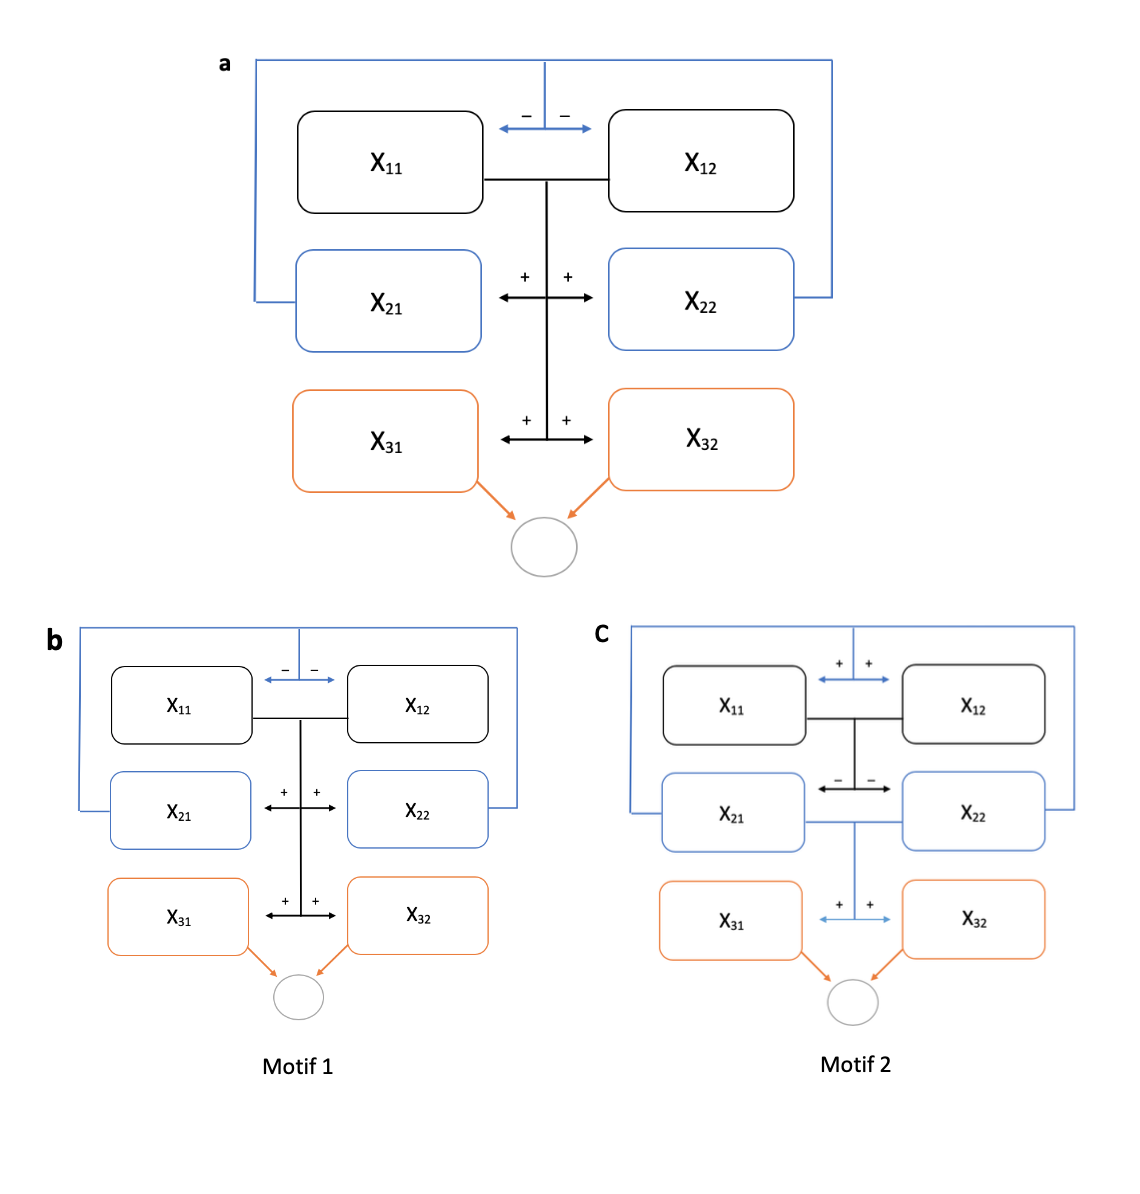
\includegraphics[scale=0.35]{../Results/Model_diagram.jpg}
    \end{center}
    \caption{Diagram showing the genetic model and two variants used to represent the migrant population. (a) Interlocus model of the population in focus. Lines labelled with mathematical symbols showing the interactions between genes. Gene $X_1$ interacts with both gene $X_2$ and $X_3$, positively regulating both of them. To limit site values below infinity, gene $X_2$ is reponsible for negatively autoregulating $X_1$. There is an output for each gene where $j = {1,2}$ and $y_j = x_{j1} + x_{j2}$. Gene $X_3$ contains the trait values for each individual, which is the output. Circle represents phenotype which is determined from trait values using a Cauchy Distribution. (b) and (c) represent models for the migrant population. (b) is the same pathway and regulation as (a) however (c) is switched where gene $X_1$ negatively autoregulates $X_2$, and gene $X_2$ positively regulates $X_1$ and $X_3$. Again, output of gene $X_3$ are the trait values used to derive fitness.}
    \label{fig:Starting parameters}
\end{wrapfigure}
Where $y_j$ is the total protein concentration at each gene. There are four sites which represent the different factors affecting protein production. These are \textit{\textalpha}, \textit{\textgamma}, \textit{\texttheta} and $P$. \textit{\textalpha} is the protein production rate while \textit{\textgamma} is the degradation rate \cite{omholt2000gene}. For both sets of populations, a single gene, $X_3$ determines the trait value for individuals and quantifiably differentiates the populations in terms of morphology \cite{orr2001genetics}. For the population in focus, gene $X_1$ positively regulates gene $X_2$ and gene $X_3$, and gene $X_1$ is negatively regulated by gene $X_2$. This is to regulate trait value and prevent the value from exceeding to infinity. As gene $X_2$ increases in expression, it decreases $X_1$ expression, negatively autoregulating the system and limiting its value. Let $j = {1,2,3}$ and $i = {1,2}$, from the separate researches of \textit{Omholt et al}(2000), and \textit{Gjuvsland et al}(2007), $R_{j}$ is a regulatory Hill Function representing a Michaelis-Menten mechanism, where $S(y_j,\theta,P) = \frac{y_j^P}{y_j^P+\theta^P}$. The Hill Function explains the relationship between regulator and producer, where \texttheta is the amount of regulator needed for 50\% production rate and P affects the steepness of the curve \cite{gjuvsland2007statistical,omholt2000gene}. Should the network be negatively regulated, it leads to the following equation:
\begin{equation*}
    R_{j}(y) = 1 - S(y, \theta_j , P_j), j = {1, 2} \label{eq:Negative autoregulation function} \tag{2}
\end{equation*}
And if positively regulated:
\begin{equation*}
	R_{j}(y) = S(y, \theta_j, P_j), j = {1, 2} \label{eq:Positive autoregulation function} \tag{3}
\end{equation*}
Again, letting $j = {1,2,3}$, as gene $X_1$ positively autoregulates gene $X_2$ and gene $X_3$, and gene $X_2$ negatively autoregulates gene $X_1$, this results in the following equations:
\begin{equation*}
    R_{1j}(y_2) = 1 – S(y_2, \theta_{2j}, P_{2j}) \label{eq:X1 negative autoregulation function} \tag{4.1},
\end{equation*}
\begin{equation*}
    R_{2j}(y_1) = 1 – S(y_1, \theta_{1j}, P_{1j}) \label{eq:X2 positive autoregulation function} \tag{4.2},
\end{equation*}
\begin{equation*}
    R_{2j}(y_1) = 1 – S(y_1, \theta_{3j}, P_{3j}) \label{eq:X3 positive autoregulation function} \tag{4.3}
\end{equation*}
\textit{\textmu} is the ratio of \textalpha and \textgamma per locus. Using the equilibrium solutions, total protein concentration is calculated by the following equations:
\begin{equation*}
    y_1 = \mu_{11}(1 – S(y_2, \theta_{21}, P_{21})) + \mu_{12}(1 – S(y_{2}, \theta_{22}, P_{22})) \label{eq:y1 function} \tag{5.1}
\end{equation*}
\begin{equation*}
    y_2 = \mu_{21}(S(y_{1}, \theta_{11}, P_{11})) + \mu_{22}(S(y_{1}, \theta_{12}, P_{12})) \label{eq:y2 function} \tag{5.2}
\end{equation*}
\begin{equation*}
    y_3 = \mu_{31}(S(y_{1}, \theta_{31}, P_{31})) + \mu_{32}(S(y_{1}, \theta_{32}, P_{32})) \label{eq:y3 function} \tag{5.3}
\end{equation*}
\subsection{Migrant network}
For the first motif, the genetic network will be the same as the main population, just evolving to a different local optimum trait value of either 65 or 80. For the second motif however, the difference is that gene $X_1$ negatively regulates gene $X_2$, while gene $X_3$ and gene $X_1$ are positively regulated by gene $X_2$. The formulas used to derive $y_1$, $y_2$ and $y_3$ values for the migrant population are as follows:
\begin{equation*}
    y_1 = \mu_{11}(S(y_2, \theta_{21}, P_{21})) + \mu_{12}(S(y_2, \theta_{22}, P_{22})) \label{eq:y1 function} \tag{6.1}
\end{equation*}
\begin{equation*}
    y_2 = \mu_{21}(1 – S(y_1, \theta_{11}, P_{11})) + \mu_{22}(1 – S(y_1, \theta_{12}, P_{22})) \label{eq:y2 function} \tag{6.2}
\end{equation*}
\begin{equation*}
    y_3 = \mu_{31}(S(y_2, \theta_{31}, P_{31})) + \mu_{32}(S(y_2, \theta_{32}, P_{32})) \label{eq:y3 function} \tag{6.3}
\end{equation*}
This is to represent the concept of differentiated species but can still integrate in the other population and interbreed.
\subsection{The simulation}
A total of 44 permutations based on conditions in \textit{(see Appendix A)} of environmental distance, genetic network structure, migration rates and migration patterns were simulated for 1,200 generations each run. For the effect of genetic drift and to account for the large deviations of values, a Cauchy distribution is used to generate fitness probabilities per generation. Since the Cauchy distribution is characterized for its heavy tails. The values entered in the Cauchy distribution are the desired trait values. It is important to note that environment is kept constant. Both populations were kept constant at 500 individuals. The main population evolved to a trait value of 50 with a standard deviation 8, while the migrant population alternated between 65 and 80 with standard deviation 10. The large standard deviations characterise the varying forms of morphology that can be noticed in species. The trait values represent the environments of both populations and the local optimums they evolve to.\\
For the simulation we assume that both populations have the same size and stay constant, with migrants replacing individuals.  There is no spatial structure and all individuals have an equal chance of being replaced. Both populations undergo divergent selection, stabilising in their own environments to different specified trait values, thus differentiating the populations over time \cite{sato2006effect}. Alleles for each individual can either be homogenous, using a uniform distribution to determine starting value between 0.1 and 0.3 for both populations, or heterogenous, using a uniform to randomly generate the starting allele values, again between 0.1 and 0.3. If the population is homogenous, each individual in the population starts with the same value at each locus, otherwise have differing values if heterogenous.
Recombination is equal chance at any locus and interchanges the alleles and everything downstream. Mutation can occur at each locus by randomly deviating from the current value. The probability is the same constant for both populations where each locus has an equal chance of mutating. Mutation probability is kept constant at 0.0011 per site. A mutation in the second gene will have trans-regulatory effects as gene $y_2$ negatively autoregulates gene $y_1$, while the effect of gene $y_1$ will affect the expression values of gene $y_3$. Since all genes in the model represent regulatory and coding regions, mutations in any site can be considered to affect phenotype, for its pleiotropic effects \cite{rice2019evolution,landry2007genetic}.\\
Fitness is reproductive success, or the probability of being a parent and passing on their allele values which is determined by phenotypic value. Each individual per generation has no limit as to how many times they can be a parent, however the standard deviation of 8 and 10 in the Cauchy distribution attempts to produce varying combination of parents. Migration rates varied between 1\%, 3\% and 5\%. As migrant individuals enter the population, they randomly replace individuals in the population. With constant population size, this represents immigration and emigration. Furthermore, low migration rates were used to prevent migration population from completely replacing the original population and allowing the network to be able to adapt to the new values. Both populations have a burn-in period of 80 generations to evolve in their own environments before migration can happen. Also, migration only occurs till the 700th generation. The remaining 500 generations are to assess how the network responds to the migration. Patterns of migration were also considered, varying between each generation, every 10 generations, every 5 generations and random (between 1\% and 5\% each occurrence) after the 80th generation.
\subsection{Analysis}
Analysis was done on the recorded fitness, trait values and population arrays. At the end of each simulation, fitness is normalised by dividing fitness probabilities with the median of Cauchy distribution for the local population, with 1.0 being the highest possible fitness value. Firstly, control conditions of no migration were simulated to see how rapidly isolated networks evolve. Without migration, I expect rapid evolution of allele values, especially for the heterogenous population due to varying alleles present \cite{garcia1997genetic}. To analyse robustness, I calculate a robustness ratio. The fittest individuals before and 10 generations after migration were recorded and replicated such that there were 4 separate mutations per site. Trait values were again inputted into the Cauchy distribution to determine fitness values. The robustness ratio is then the variance in fitness after migration divided by variance in fitness before migration. Ratios were then log transformed as to linearise and make it less skewed. A negative value is thus desired for robustness and analysis of variance test is done to see if any factors significantly contribute to robustness.
